\documentclass{article}


% if you need to pass options to natbib, use, e.g.:
%     \PassOptionsToPackage{numbers, compress}{natbib}
% before loading neurips_2022


% ready for submission
% \usepackage{neurips_2022}


% to compile a preprint version, e.g., for submission to arXiv, add add the
% [preprint] option:
%     \usepackage[preprint]{neurips_2022}


% to compile a camera-ready version, add the [final] option, e.g.:
    \usepackage[final]{neurips_2022}


% to avoid loading the natbib package, add option nonatbib:
%    \usepackage[nonatbib]{neurips_2022}


\usepackage[utf8]{inputenc} % allow utf-8 input
\usepackage[T1]{fontenc}    % use 8-bit T1 fonts
\usepackage{hyperref}       % hyperlinks
\usepackage{url}            % simple URL typesetting
\usepackage{booktabs}       % professional-quality tables
\usepackage{amsfonts}       % blackboard math symbols
\usepackage{nicefrac}       % compact symbols for 1/2, etc.
\usepackage{microtype}      % microtypography
\usepackage{xcolor}         % colors
\usepackage{color,soul}
\usepackage{hyperref}
\usepackage{titling}
\usepackage{graphicx}
\title{Weight-based Modality Fusion for Multimodal Digit Recognition}


% The \author macro works with any number of authors. There are two commands
% used to separate the names and addresses of multiple authors: \And and \AND.
%
% Using \And between authors leaves it to LaTeX to determine where to break the
% lines. Using \AND forces a line break at that point. So, if LaTeX puts 3 of 4
% authors names on the first line, and the last on the second line, try using
% \AND instead of \And before the third author name.


\author{%
  Chonglin Zhang\\
  833003072 \\
  Computer Science Department\\
  Texas A$\&$M University\\
  College Station, TX 77845 \\
  Kaggle Team Name: Chonglin Zhang \\
  \texttt{czhang71@tamu.edu} \\
}


\begin{document}

\maketitle


\begin{abstract}
  Multimodal Digit Recognition involves the task of recognizing digits using both handwritten digit images and speech signals. This task explores the fusion of multiple sources of information to enhance the accuracy and robustness of digit recognition systems. In this paper, we propose a weight-based modality fusion method. This method learns a unique weight for each modality and then fuses the modalities based on these weights to obtain fused features, thereby improving the model's performance. Our approach achieved a macro F1 score of 0.992 on multimodal MNIST, surpassing previous benchmarks. Furthermore, a series of ablation experiments demonstrate that our method outperforms single-modal approaches.
\end{abstract}


\section{Introduction}
Digit recognition systems have wide-ranging applications in real-world scenarios such as human-computer interaction and biometric security. Traditional methods rely on a single modality to recognize digits, such as identifying handwritten digits from images. However, this approach encounters difficulties when the handwritten digit images are unclear and lack additional information for context. Multimodal digit recognition addresses this challenge by leveraging additional modalities. For instance, when the handwritten image is unclear, associated speech signals can provide supplementary context for accurate recognition. The challenge of multimodal digit recognition lies in how to integrate features from different modalities to produce more accurate and robust results.

In this paper, we propose a weight-based fusion method to address this challenge. Specifically, we construct a simple model for each modality to encode its features, resulting in feature representations for each modality. Additionally, we learn a separate weight for each modality. Subsequently, we combine each modality based on their respective weights to obtain the final fused features, which are then used for classification. We tested our method on the multimodal MNIST dataset and achieved a macro F1 score of 0.992.


\section{Method}

\begin{figure*}[!t]
	\begin{center}

		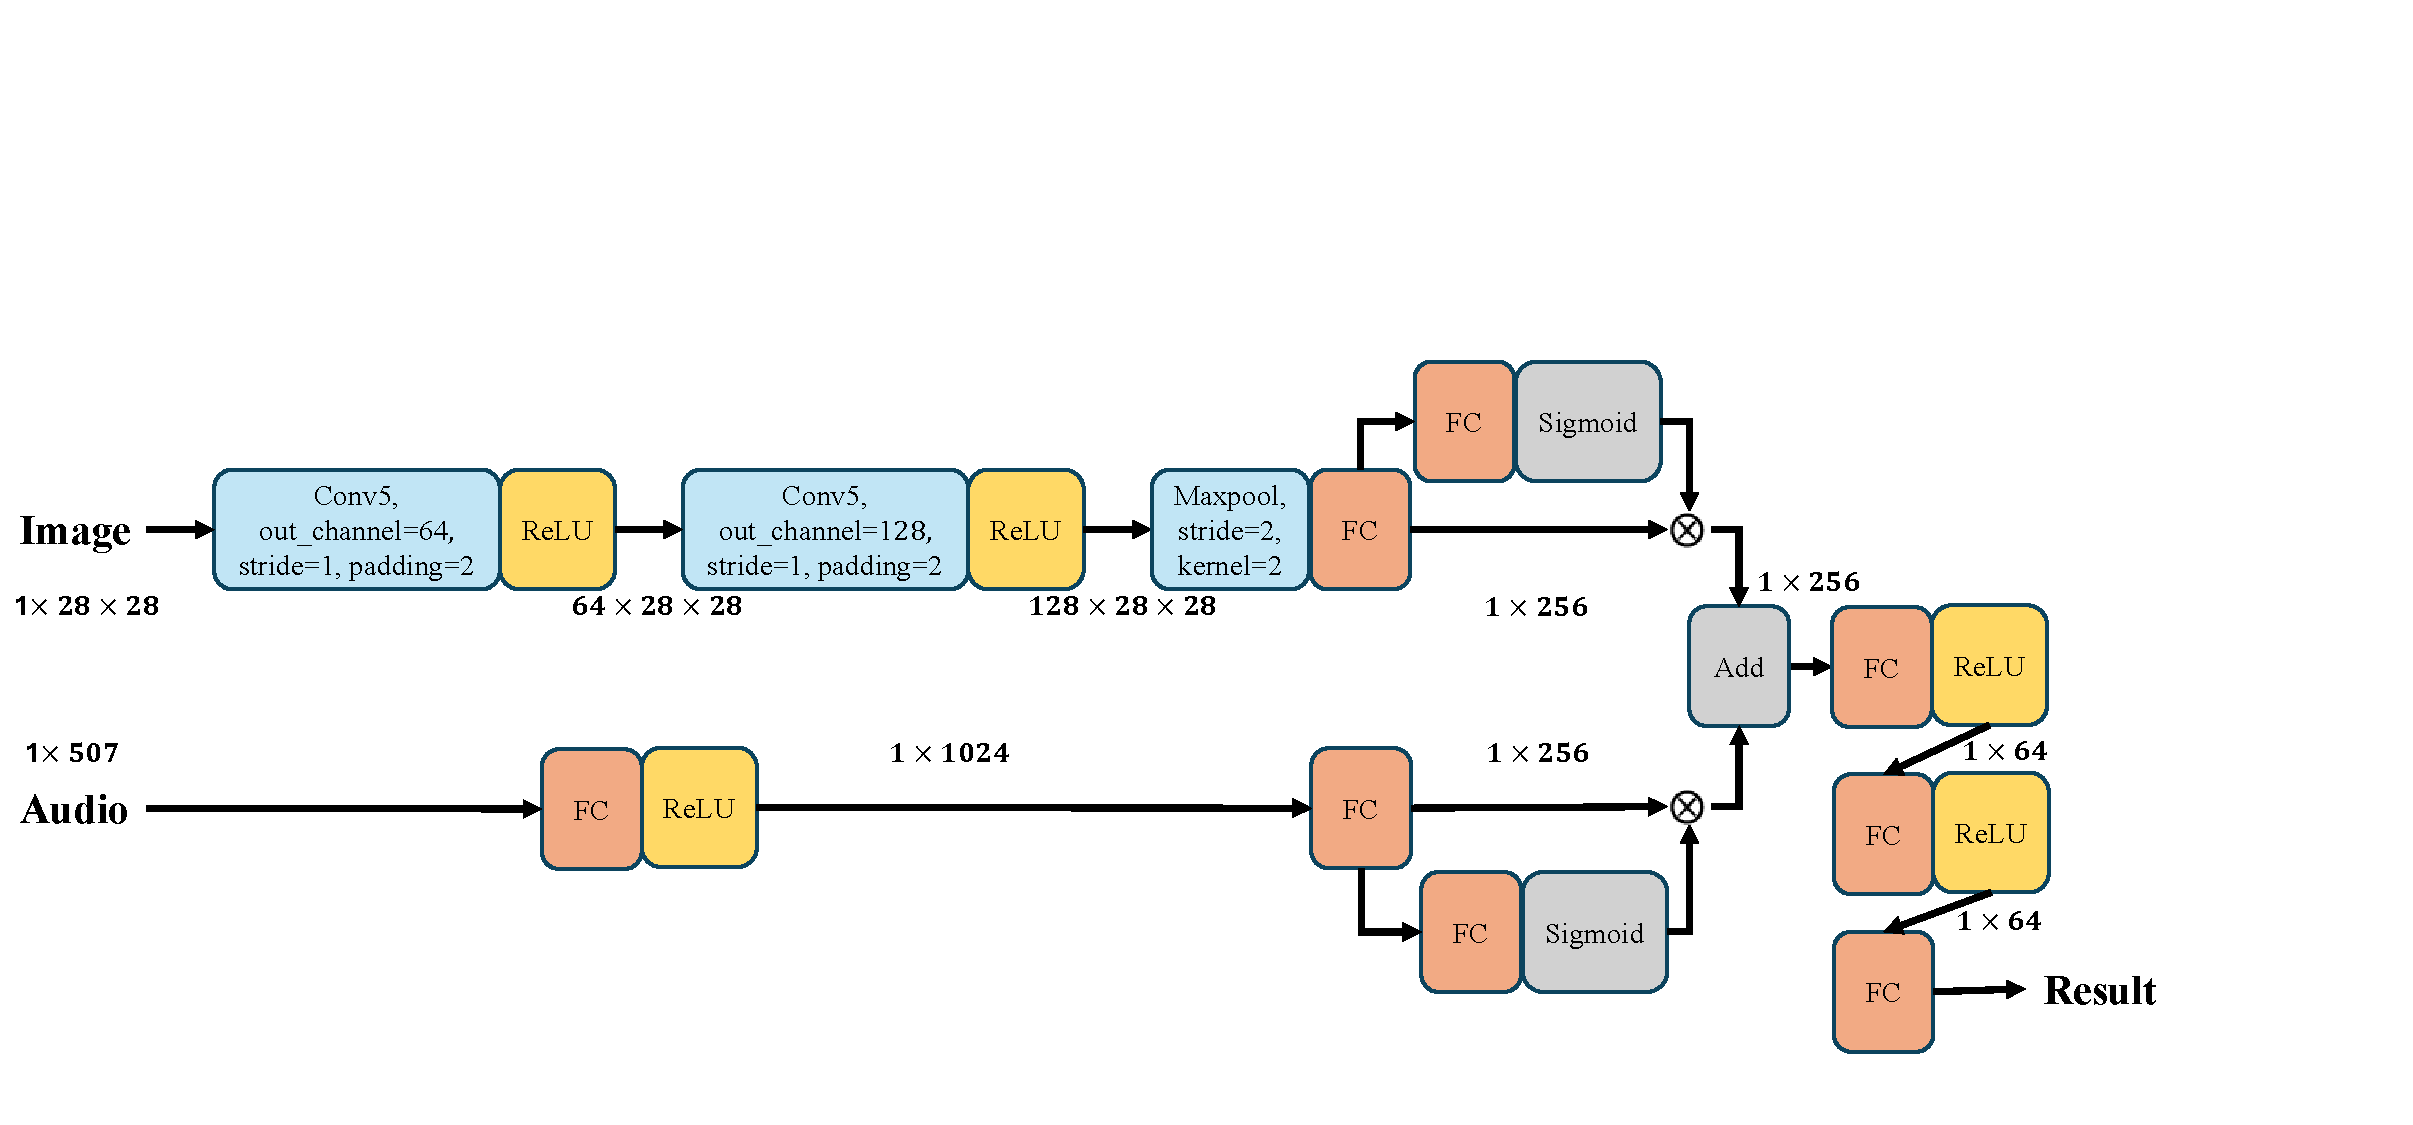
\includegraphics[width=0.90\textwidth]{overview.pdf}
	\end{center}
	\caption{The overall structure of our proposed method, where $\otimes$ denotes element-wise multiplication, and \textit{Add} denotes element-wise addition.} 
	\label{fig:overview}
\end{figure*}

The overall structure of our method is illustrated in Figure~\ref{fig:overview}. We first extract features from each modality and then fuse them using a weight-based method to obtain fused features. Finally, we use these fused features to derive the final classification results.

\subsection{Data Preprocessing}

We performed preprocessing on the image data. For each sample, we resized it to $28\times 28$ dimensions and then divided all pixel values by 255 to normalize them between 0 and 1. This was done for ease of computation during backpropagation and to prevent gradients from becoming too large. As for the speech signal data, since it was already in the range of 0 to 1, we did not perform any further preprocessing on it.

We divided all the data into 80\% for the training set and the remaining 20\% for the validation set.
\subsection{Model Design}

The specific details of our model are illustrated in Figure~\ref{fig:overview}. For the image data, we employed a convolutional neural network (CNN) to extract features. We experimented with various CNN model designs in HW4, including changing kernel sizes, activation functions, adding or removing dropout layers, etc. Consequently, we directly adopted the best-performing model from HW4 as the feature extraction network for images. We removed the final classification layer from the model, resulting in each sample being encoded into a $256$-dimensional feature vector.

As for the speech data, since it is a one-dimensional signal, we employed fully connected (FC) layers to extract features. Similarly, we used 2 layers of FC networks to encode each sample into a $256$-dimensional feature vector.

During the fusion stage, we learned a weight for each modality. Specifically, for each modality, we passed its features through an FC layer with a single output to obtain a weight. These weights were then mapped to the range of 0 to 1 using a sigmoid function. Subsequently, we multiplied each modality's features by its corresponding weight and summed them to obtain the fused feature. The fused feature was then passed through 3 layers of FC networks to obtain the final output.
\subsection{Model Training}

We constructed our model using PyTorch. For the loss function, we employed the commonly used cross-entropy loss for classification tasks. The model was trained using the SGD optimizer for a total of 40 epochs.

\subsection{Hyperparameter Tuning}

For the SGD optimizer, we set the momentum to 0.9 and weight decay to 0.0001. The initial learning rate was set to 0.01 and decreased by a factor of 10 every 10 epochs. During training, the batch size was set to 64.

\section{Results}

\subsection{Dataset}
We conducted experiments on the Multimodal MNIST dataset to validate our method. Each sample in the Multimodal MNIST dataset consists of both image and speech modalities. The dataset contains a total of 60,000 samples for training. We used 80\% of the dataset for training and the remaining 20\% for validation.We used the macro F1 score as the evaluation metric to assess the models.

\subsection{Ablation Study}

\begin{table}[!htb]
	\caption{Comparison of Different Feature Fusion Methods on Multimodal MNIST.}
	\label{tab:ablation}
	\centering
	\begin{tabular}{c|c}
		\toprule
		Fusion Method        & F1 socre \\
		\midrule
		Image & 0.991    \\
		Audio & 0.752    \\
		Add w/o weights & 0.991    \\
		Add w/ weights & 0.992   \\
		\bottomrule
	\end{tabular}
\end{table}

We conducted experiments on various feature fusion methods, and the results are shown in Table~\ref{tab:ablation}. Multimodal fusion yielded better results compared to single modality approaches. Furthermore, the weight-based addition method outperformed the direct addition fusion method.

\subsection{Comparison with Other Methods}

\begin{table}[!htb]
	\caption{Comparison with Other Methods on Multimodal MNIST.}
	\label{tab:result}
	\centering
	\begin{tabular}{c|c}
		\toprule
		Method        & F1 socre \\
		\midrule
		benchmark\_01 & 0.606    \\
		benchmark\_02 & 0.886    \\
		benchmark\_03 & 0.952    \\
		\midrule
		\textbf{Ours}          & \textbf{0.992}   \\
		\bottomrule
	\end{tabular}
\end{table}

The experimental results are shown in Table~\ref{tab:result}. Our method achieved a macro F1 score of 0.992, surpassing all previous benchmarks, thus validating the effectiveness of our approach.

\subsection{Visualization}

\begin{figure*}[!htb]
	\begin{center}
		
		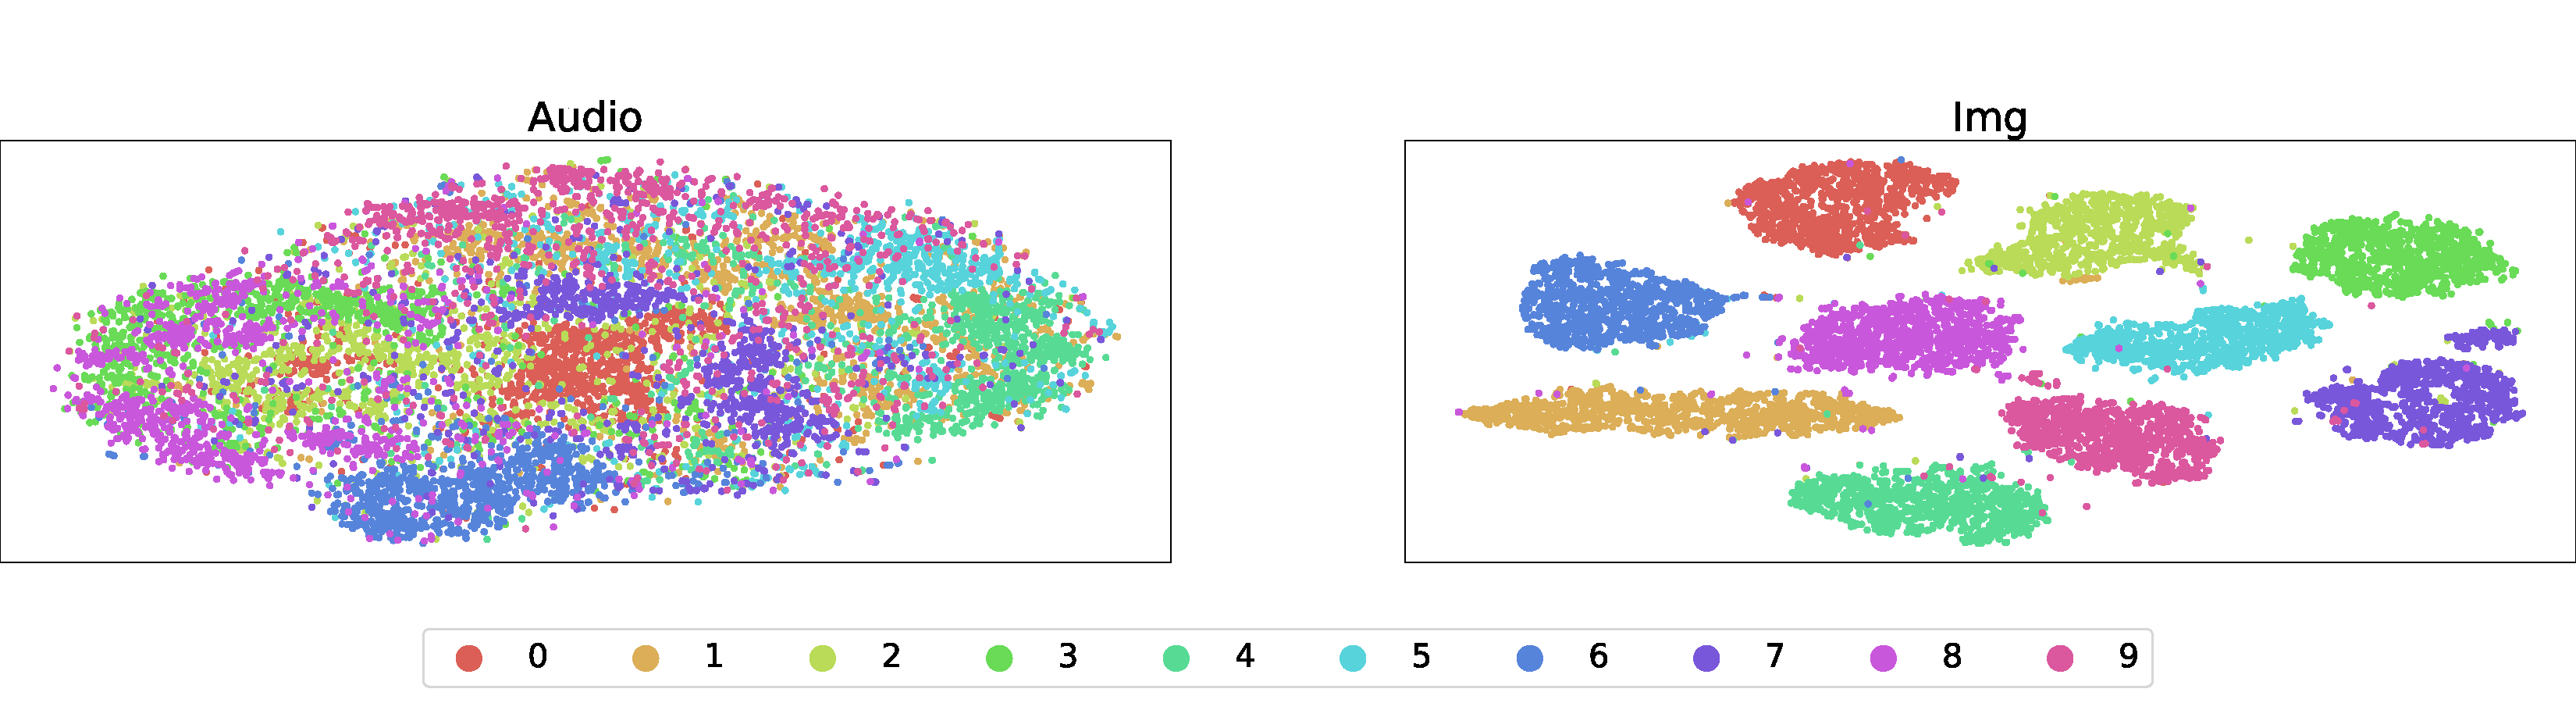
\includegraphics[width=0.90\textwidth]{tsne.pdf}
	\end{center}
	\caption{Visualization of Speech and Image Features.} 
	\label{fig:visualization}
\end{figure*}

To further evaluate the contribution of different modalities to the model, we visualized the features of the image and speech modalities separately. We used t-SNE to visualize the features extracted by the model on the validation set for both image and speech modalities. The results are shown in Figure~\ref{fig:visualization}.

In the visualization of image features, the clusters for each category are distinct and well-separated. In contrast, the visualization of speech features shows less distinct separation between clusters for each category, leading to potential confusion.

The visualizations further support the results in Table~\ref{tab:ablation} regarding the performance of individual modalities. We hypothesize that this outcome may be due to handwritten image data being more easily recognizable compared to speech signals. Additionally, another reason could be the simplicity of our speech feature extraction model.

\section{Conclusion}

In this study, we proposed a weight-based fusion method for multimodal digit recognition. Our experimental results on the Multimodal MNIST dataset demonstrate that our approach outperforms single-modal methods and other fusion techniques, achieving a macro F1 score of 0.992.

However, our method still has some limitations, notably in the simplicity of the speech feature extraction model, which may not sufficiently extract high-quality features. In future work, we plan to design more sophisticated speech feature extraction models to improve feature extraction capabilities, thus enhancing the accuracy and robustness of the model.


\end{document}
